\documentclass[conference]{IEEEtran}

\usepackage{newtxtext,newtxmath}
\usepackage{amsmath}
\usepackage{booktabs}
\usepackage{graphicx}
\usepackage{longtable}
\usepackage{array}
\usepackage{url}
\usepackage[hidelinks]{hyperref}
\usepackage{tikz}
\usetikzlibrary{arrows.meta}

\urlstyle{tt}
\setlength{\emergencystretch}{3em}
\newcolumntype{L}[1]{>{\raggedright\arraybackslash}p{#1}}
\newcommand{\codepath}[1]{{\Urlmuskip=0mu plus 1mu\relax\nolinkurl{#1}}}

\begin{document}

\title{Geo-Distributed Data Center Scheduling to Smooth Grid Ramps and Reduce Monthly Net-Load Peaks}

\author{\IEEEauthorblockN{Janusz Gal}
\IEEEauthorblockA{jgal@charlotte.edu}}

\maketitle

\begin{IEEEkeywords}
data centers, demand response, grid ramp, net-load peak, reinforcement learning,
workload scheduling
\end{IEEEkeywords}

\section{Introduction and Scope}
\label{sec:introduction}

Large data centers draw enough electrical power that the timing and location 
of their computing work matter to the grids that serve them. Some work must
run immediately, while lower-priority work may be delayed. An operator with
multiple sites may also choose where that work runs.

The question we ask here is:
\begin{quote}
\emph{How much can a causal scheduler jointly smooth normalized one-hour
regional net-load ramps and reduce regional monthly net-load peaks, using temporal deferral and geographic
routing while satisfying immediate-service, batch-window, and site-capacity
constraints?}
\end{quote}

We use Google workload traces and EIA grid data to model a synthetic fleet
of four data centers. Each hour, the scheduler chooses where service runs,
how much batch work to execute, and where to execute it. We will use
proximal policy optimization (PPO) to train a policy that minimizes an equally
weighted combination of scaled monthly ramp impact and regional peaks while meeting
workload deadlines and site-capacity limits.

\section{Google ClusterData2019 Workload Trace}
\label{sec:clusterdata2019}

\subsection{Dataset}
\label{subsec:clusterdata-role}

A \emph{Borg cell} is a group of machines managed as one computing cluster.
Google provides records for eight cells, labeled \(a\)--\(h\), from May 2019
\cite{wilkes2020clusterdata2019, tirmazi2020borg}. The trace includes machine
capacity, per-instance resource usage, collection events, priorities, and
resource requests. It is sanitized: it contains no user, application,
location, or other identifying information.

Three tables supply the workload data used here: \codepath{machine_events}
for the CPU reference capacity, \codepath{instance_usage} for measured CPU
execution, and \codepath{collection_events} for
priority.\footnote{The full trace is approximately 2.4 TiB, so the extraction
queries it through BigQuery rather than downloading it.}

Rather than track individual jobs and their execution, we use the aggregate CPU utilization (for each five-minute window) as our demand.   

\begin{figure}[!ht]
  \centering
  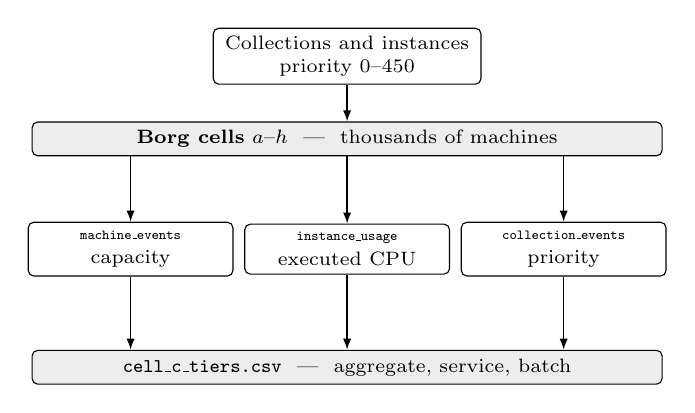
\begin{tikzpicture}[
    font=\scriptsize,
    box/.style={draw, rounded corners=2pt, align=center, inner sep=3pt},
    shaded/.style={box, fill=black!7},
    arr/.style={-{Latex[length=1.4mm]}, semithick}
  ]
    \node[box, minimum width=34mm] (jobs) at (0,0)
      {Collections and instances\\priority 0--450};

    \node[shaded, minimum width=80mm] (cell) at (0,-1.05)
      {\textbf{Borg cells} \(a\)--\(h\)\ \ ---\ \ thousands of machines};

    \node[box, minimum width=26mm] (me) at (-2.75,-2.45)
      {\texttt{\tiny machine\_events}\\[1pt]capacity};
    \node[box, minimum width=26mm] (iu) at (0,-2.45)
      {\texttt{\tiny instance\_usage}\\[1pt]executed CPU};
    \node[box, minimum width=26mm] (ce) at (2.75,-2.45)
      {\texttt{\tiny collection\_events}\\[1pt]priority};

    \node[shaded, minimum width=80mm] (csv) at (0,-3.95)
      {\texttt{cell\_c\_tiers.csv}\ \ ---\ \ aggregate, service, batch};

    \draw[arr] (jobs) -- (cell);
    \draw[arr] (cell.south -| me) -- (me.north);
    \draw[arr] (cell.south -| iu) -- (iu.north);
    \draw[arr] (cell.south -| ce) -- (ce.north);
    \draw[arr] (me.south) -- (me.south |- csv.north);
    \draw[arr] (iu.south) -- (iu.south |- csv.north);
    \draw[arr] (ce.south) -- (ce.south |- csv.north);
  \end{tikzpicture}
  \caption{Extraction path from the Google trace to the retained five-minute
  tier curves. The symbol \(c\) identifies a Google cell.}
  \label{fig:clusterdata-pipeline}
\end{figure}

\subsection{Fixed reference capacity}
\label{subsec:clusterdata-capacity}

Google expresses CPU capacity in normalized units, with the largest machine (in a cell)
equal to 1.0. We then define a cell's reference capacity is the sum over its machines:
\begin{equation}
  C^{\mathrm{ref}}_c
  =
  \sum_{n\in\mathcal{J}_c}\kappa_n ,
  \label{eq:reference-capacity}
\end{equation}
where \(\mathcal{J}_c\) is all machines ever observed in cell \(c\)
and \(\kappa_n\) is machine \(n\)'s largest reported
\codepath{capacity.cpus}.\footnote{Machines can have multiple add, update,
and snapshot records in \codepath{machine_events}; we keep the largest
reported capacity. This gives a fixed monthly reference, rather than the
active capacity in each five-minute interval.}

\subsection{Five-minute executed CPU}
\label{subsec:clusterdata-utilization}

For each five-minute window, we sum recorded CPU usage and divide by the
cell's fixed reference capacity. Let \(k\) identify the window and
\(\mathcal{E}_{c,k}\) denote its set of retained usage rows:
\begin{equation}
  u_{c,k}
  =
  \frac{\displaystyle\sum_{r\in\mathcal{E}_{c,k}} a_r}
         {C^{\mathrm{ref}}_c} ,
  \label{eq:clusterdata-utilization}
\end{equation}
where \(a_r\) is row \(r\)'s \codepath{average_usage.cpus} value. Both the
numerator and denominator use Google's normalized CPU units, so
\(u_{c,k}\) is dimensionless.

We retain only top-level instances and rows covering at least one full five-minute
interval.\footnote{Top-level instances are rows whose
\codepath{alloc_collection_id} is null or zero. Restricting to them follows
Google's own analysis example and avoids counting both an allocation set and
the work running inside it \cite{googleTraceFormatV3,
googleClusterAnalysisColab}. The second filter removes rows with
\codepath{end_time}\,\(-\)\,\codepath{start_time} below 300 s so that every
retained row spans a complete bucket; a retained row is assigned to the
bucket containing its start time.}

\subsection{Modeled service and batch classes}
\label{subsec:clusterdata-tier-split}

Google records job priorities rather than explicit service and batch
labels. We use the priority bands from Google's analysis in
Table~\ref{tab:priority-bands} and assume work in the no-SLO bands can be
deferred.\footnote{Priority comes from \codepath{collection_events}. We keep
\codepath{type=0} events, take the highest priority recorded for each
\codepath{collection_id}, and join that to the usage rows.}

\begin{table}[htbp]
  \centering
  \footnotesize
  \caption{ClusterData2019 priority bands used by the extraction.}
  \label{tab:priority-bands}
  \begin{tabular}{@{}llr@{}}
    \toprule
    Band & Interpretation in source & Priority \\
    \midrule
    Free & no-SLO & 0--99 \\
    Best-effort batch & no-SLO & 100--115 \\
    Mid & higher priority & 116--119 \\
    Production & higher priority & 120--359 \\
    Monitoring & higher priority & 360 and above \\
    \bottomrule
  \end{tabular}
\end{table}

We classify priority 115 or below as batch and the remaining usage as
service. Let \(p_r\) be the priority attached to row \(r\), and
\(\mathcal{E}^{\mathrm{bat}}_{c,k}\) the set of rows in
\(\mathcal{E}_{c,k}\) with \(p_r\leq115\).\footnote{Usage rows without a
matching priority record remain in the service residual.} The two classes are
\begin{align}
  u^{\mathrm{bat}}_{c,k}
  &=
  \frac{1}{C^{\mathrm{ref}}_c}
  \sum_{r\in\mathcal{E}^{\mathrm{bat}}_{c,k}} a_r,
  \label{eq:batch-utilization}\\
  u^{\mathrm{svc}}_{c,k}
  &=
  u_{c,k}-u^{\mathrm{bat}}_{c,k}.
  \label{eq:service-utilization}
\end{align}
We refer to these curves as \emph{deferrable batch} and
\emph{nondeferrable service}. Four cells supply the workload profiles, which
are converted to hourly arrivals in Section~\ref{sec:data-transformations}.
Appendix~\ref{app:data-schemas} lists the stored columns and example values.

\section{Google PowerData2019 Server-Power Model}
\label{sec:powerdata2019}

\subsection{Data fit}
\label{subsec:powerdata-purpose}

PowerData2019 \cite{googlePowerData2019} provides five-minute normalized
server-power measurements for the same Borg cells. We average
\codepath{measured_power_util} and normalized CPU execution by hour, then
fit an ordinary least-squares line:
\begin{equation}
  \widehat p_c(u)
  =
  \alpha_c+\beta_c u.
  \label{eq:powerdata-affine-fit}
\end{equation}
The intercept \(\alpha_c\) represents idle power, and \(\beta_c\) describes
how power increases with utilization. The fitted idle draw ranges from
about 38\% to 55\% of reference power across the cells.

\subsection{Active coefficients and power range}
\label{subsec:powerdata-coefficients}

Table~\ref{tab:powerdata-coefficients} lists the fitted coefficients for the
four cells used here.\footnote{Stored in
\codepath{data/power_model_params.json}.} Google reports normalized power,
so we assume a reference power of 500 MW per site. At this scale, modeled
idle power ranges from 191 to 274 MW, with full utilization adding
170 to 285 MW, depending on the cell.

\begin{table*}[htbp]
  \centering
  \small
  \caption{CPU-only power fits at the 500 MW reference scale.}
  \label{tab:powerdata-coefficients}
  \begin{tabular}{@{}crrrcrrr@{}}
    \toprule
    Cell & \(\alpha_c\) & \(\beta_c\) & \(R^2\) & Observed \(u\)
         & \(u=0\) & \(u=1\) & Swing \\
         & & & & & \multicolumn{3}{c}{MW} \\
    \midrule
    \(a\) & 0.528016 & 0.339728 & 0.7885 & 0.363--0.682
          & 264 & 434 & 170 \\
    \(b\) & 0.548190 & 0.375761 & 0.7479 & 0.415--0.654
          & 274 & 462 & 188 \\
    \(c\) & 0.439604 & 0.525740 & 0.7642 & 0.397--0.667
          & 220 & 483 & 263 \\
    \(d\) & 0.382039 & 0.570370 & 0.8005 & 0.346--0.627
          & 191 & 476 & 285 \\
    \bottomrule
  \end{tabular}
\end{table*}



\section{Grid, Market, and Forecast Data}
\label{sec:energy-data}

\subsection{Four market cases}
\label{subsec:energy-sources}

Each modeled site is assigned to an electricity market. We use hourly
demand and generation by fuel from the EIA grid monitor
\cite{eiaGridMonitor}. CAISO NP15 draws on the CISO balancing authority,
MISO Minnesota on MISO, SPP North on SWPP, and ISO-NE NEMA on ISNE.

For each region, we use demand, wind generation, and solar
generation.\footnote{The EIA fields \codepath{D},
\codepath{NG.WND}, and \codepath{NG.SUN} are stored as
\codepath{gross_demand_mw}, \codepath{wind_mw}, and \codepath{solar_mw}.}
EIA labels each interval by its ending hour. We subtract one hour to store
hour-beginning UTC timestamps, giving one row per market per hour.

\subsection{Net load}
\label{subsec:energy-net-load}

Net load is demand minus wind and solar generation. Let \(\tau\) be a UTC
hour, \(D_m\) demand, and \(G^{\mathrm{wnd}}_m\), \(G^{\mathrm{sol}}_m\)
observed wind and solar output, all in MW:
\begin{equation}
  N_m(\tau)
  =
  D_m(\tau)
  -G^{\mathrm{wnd}}_m(\tau)
  -G^{\mathrm{sol}}_m(\tau).
  \label{eq:energy-net-load}
\end{equation}




\subsection{Calendar and frozen statistics}
\label{subsec:energy-calendar}

We use 2025 grid data. The training set, \(\mathcal E_{\mathrm{train}}\),
contains the eleven months outside May (334 UTC days). May (31 UTC days)
is used for validation. Each month is a continuous simulation, as
described in Section~\ref{subsec:transform-pairing}.

To compare markets of different sizes, we define a fixed scale
\(S_m\) for each market: the empirical 95th percentile of gross demand over
the training months,
\begin{equation}
  S_m
  =
  Q_{0.95}\!\left(\{D_m(\tau):\tau\in\mathcal{R}\}\right),
  \label{eq:market-scale}
\end{equation}
where \(\mathcal{R}\) is every hour of 2025 outside May.
The scales in Table~\ref{tab:frozen-stats} are held fixed throughout training
and validation. We use them to express net-load ramps and peaks relative to
each market's demand scale.

\begin{table}[htbp]
  \centering
  \footnotesize
  \caption{Regional normalization scale \(S_m\), in MW.}
  \label{tab:frozen-stats}
  \begin{tabular}{@{}lr@{}}
    \toprule
    Market case & \(S_m\) \\
    \midrule
    CAISO NP15     & 33,983 \\
    MISO Minnesota & 101,250 \\
    SPP North      & 46,367 \\
    ISO-NE NEMA    & 18,007 \\
    \bottomrule
  \end{tabular}
\end{table}

\subsection{Forecasts}
\label{subsec:energy-forecasts}

Each row contains gross-demand and net-load predictions with lead times of
one, three, six, and twelve hours from its issue time. The decision at hour
\(t\) reads the forecasts issued at \(t-1\), so their targets are
\(t\), \(t+2\), \(t+5\), and \(t+11\): the current decision hour and
two, five, and eleven hours later. Queue urgency is reported separately as
work due within one, three, six, twelve, and twenty-four execution slots.

We generate these forecasts from EIA data using linear regressions. Inputs
available at the issue hour include recent demand, demand at the same hour
yesterday and a week earlier, recent one-hour and three-hour changes, and
wind and solar generation.\footnote{Generated
by \codepath{scripts/build_causal_forecasts.py}. Each market has a separate
model for each quantity and each of the four lead times, thirty-two in all.
Model fitting uses the eleven training months, excluding May.}
Section~\ref{subsec:problem-causality} gives the full list of information
available at each decision.


The hourly grid panels contain demand, wind and solar generation, net load,
the fixed market scale, and forecasts for each market.
Appendix~\ref{app:data-schemas} lists the columns and an example row.

\section{The Synthetic Four-Site Fleet}
\label{sec:data-transformations}

\subsection{Cell-to-market mapping and standardized work}
\label{subsec:transform-mapping}

We assume the fixed cell-to-market mapping in
Table~\ref{tab:active-market-map}; Google does not report cell locations.
The site index \(m\) therefore identifies the source cell for its workload
curves \(u^{\mathrm{svc}},u^{\mathrm{bat}}\) and power coefficients
\(\alpha_m,\beta_m\). All four sites have compute capacity \(K_m=1\) and
reference power \(\overline P_m=500\) MW.

\begin{table}[htbp]
  \centering
  \footnotesize
  \caption{Source cell for each modeled site, named by its market case.}
  \label{tab:active-market-map}
  \begin{tabular}{@{}ll@{}}
    \toprule
    Market case & Source cell \\
    \midrule
    CAISO NP15     & \(a\) \\
    MISO Minnesota & \(b\) \\
    SPP North      & \(c\) \\
    ISO-NE NEMA    & \(d\) \\
    \bottomrule
  \end{tabular}
\end{table}

Decisions are hourly, so \(\Delta t=1\) h. One work unit means
\emph{one site running at full utilization for one hour}; 0.5 work units
means half utilization for that hour. Although sites share this capacity and
the 500 MW reference scale, their different power coefficients
\(\alpha_m,\beta_m\) mean the same work can draw different power at each site.

\subsection{Pairing repeated workload with grid time}
\label{subsec:transform-pairing}

The 744-hour Google workload restarts at the beginning of each calendar
month; shorter months use only the hours they need. The same workload is
used in the eleven training months and the May validation month.

Each month is an independent, continuous simulation. Queues and site-power
history carry across midnight, and every decision hour is scored. The
decision hours for month \(e\) are \(\mathcal T_e=\{0,\ldots,T_e-1\}\), where
\(T_e\) is its length in hours. One preceding hour,
\(\mathcal W=\{-1\}\), initializes the grid and site-power history for the
first decision and ramp calculation.
Its power is computed by executing the preceding workload in place;
that warm-up work is not added to the queues. The warm-up hour is excluded
from monthly peak maxima.

Queues start empty and must be empty at month-end. Arrivals in the final
23 hours receive shorter completion windows under
Equation~\eqref{eq:batch-deadline}.

Let \(s_{m,t}\) and \(q_{m,t}\) denote hourly service and batch arrivals at
site \(m\). Service must run immediately; batch may wait.

We convert the five-minute utilization curves from
Section~\ref{sec:clusterdata2019} to work by averaging the twelve windows in
each hour, then multiplying by the site's hourly capacity
\(K_m\Delta t\).\footnote{We treat each hour's recorded CPU execution as
work arriving at the start of the corresponding simulation hour. For
example, average utilization of 60\% becomes 0.6 work units.} Let \(t\)
be the hour within the month:
\begin{align}
  s_{m,t}
  &=
  \frac{K_m\Delta t}{12}
  \sum_{b=0}^{11} u^{\mathrm{svc}}_{m,12t+b},
  \label{eq:synthetic-service-arrivals}\\
  q_{m,t}
  &=
  \frac{K_m\Delta t}{12}
  \sum_{b=0}^{11} u^{\mathrm{bat}}_{m,12t+b}.
  \label{eq:synthetic-batch-arrivals}
\end{align}
With \(K_m=1\) work unit per hour
and \(\Delta t=1\) h, the resulting work amounts equal the hourly average
utilization values numerically.

We use grid data from the corresponding UTC hours. If \(\tau_e\) is the
month's UTC start time,
\begin{equation}
  \begin{aligned}
    D_{m,t} &= D_m(\tau_e+t\Delta t), \\
    N_{m,t} &= N_m(\tau_e+t\Delta t).
  \end{aligned}
  \label{eq:episode-grid-map}
\end{equation}
This mapping also applies to the preceding warm-up hour.

\subsection{Available control scale}
\label{subsec:transform-control-authority}

At the 500 MW reference scale, the sum of the four individual idle-to-full
server-power ranges is approximately 906 MW. Table~\ref{tab:workload-feasibility} summarizes the repeated 744-hour
workload. 

\begin{table}[htbp]
  \centering
  \footnotesize
  \caption{Fleet workload statistics in standardized work units.}
  \label{tab:workload-feasibility}
  \begin{tabular}{@{}lrrr@{}}
    \toprule
    Quantity & Median & Q95 & Maximum \\
    \midrule
    Service arrivals & 1.723 & 1.971 & 2.090 \\
    Batch arrivals   & 0.440 & 0.602 & 0.779 \\
    Total arrivals   & 2.197 & 2.364 & 2.424 \\
    \bottomrule
  \end{tabular}
\end{table}

For grid context, Table~\ref{tab:native-ramp-scale} reports absolute one-hour
original grid ramps over the 334 training days. These are raw MW changes; the
objective later divides by \(S_m\Delta t\) to express them as fractions of
each market's demand scale per hour.
Against the median one-hour original ramp, a site's idle-to-full power range
is 19\% in CAISO NP15,
11\% in MISO Minnesota, 33\% in SPP North, and 64\% in ISO-NE NEMA; against
the Q90 ramp these ranges fall to between 4\% and 26\%. The site's power
range is a larger fraction of typical ramps than extreme ramps, particularly
in the smaller markets.

\begin{table}[htbp]
  \centering
  \footnotesize
  \caption{Absolute one-hour original net-load ramp magnitudes over training
  hours, in MW.}
  \label{tab:native-ramp-scale}
  \begin{tabular}{@{}lrr@{}}
    \toprule
    Market case & Median & Q90 \\
    \midrule
    CAISO NP15     & 900   & 4,144 \\
    MISO Minnesota & 1,691 & 4,396 \\
    SPP North      & 805   & 2,453 \\
    ISO-NE NEMA    & 445   & 1,102 \\
    \bottomrule
  \end{tabular}
\end{table}


\section{Problem Statement}
\label{sec:problem-statement}

\subsection{Sets, inputs, and units}
\label{subsec:problem-given-inputs}

Let \(\mathcal M=\{1,\ldots,4\}\) be the modeled sites and their paired market
cases. Indices \(i\) and \(j\) identify batch origin and execution
destination, respectively. Let
\(\mathcal T_e=\{0,\ldots,T_e-1\}\) be the decision-slot indices of simulated
month \(e\) with \(T_e\) hours, and \(\mathcal W=\{-1\}\) the preceding warm-up
slot. One interval has duration \(\Delta t=1\) h. The month index is omitted
from hourly quantities.

For each site and hour, the model uses synthetic service arrivals
\(s_{m,t}\), synthetic batch arrivals \(q_{m,t}\), standardized compute
capacity \(K_m\), reference power \(\overline P_m\), power coefficients
\(\alpha_m,\beta_m\), the batch window \(H\), regional net load \(N_{m,t}\),
and training-only scale \(S_m\).

Work can be divided among sites. We do not model individual jobs, memory
limits, machine types, application dependencies, or scheduling within a site.

\subsection{Scheduler controls}
\label{subsec:problem-decisions}

Each hour, the scheduler chooses:
\begin{enumerate}
  \item \(x^{\mathrm{svc}}_{j,t}\), service executed at destination \(j\);
  \item \(z_t\), total queued batch work executed now; and
  \item \(x^{\mathrm{bat}}_{j,t}\), that batch total divided by destination.
\end{enumerate}

\subsection{Immediate service}
\label{subsec:problem-service}

All service arrivals must execute in the same hour; the scheduler chooses
where:
\begin{equation}
  \sum_{j\in\mathcal M}x^{\mathrm{svc}}_{j,t}
  =
  \sum_{m\in\mathcal M}s_{m,t},
  \qquad
  x^{\mathrm{svc}}_{j,t}\geq0.
  \label{eq:service-conservation}
\end{equation}


\subsection{Batch queue and deadlines}
\label{subsec:problem-batch}

The scheduler chooses how much batch work to execute and distributes it
among sites with available capacity. Its execution site determines its
power consumption. Let \(z_t\) be the total release, \(y_{i,t}\) the work
released from origin \(i\)'s backlog, and \(x^{\mathrm{bat}}_{j,t}\) the work
executed at destination \(j\). Released work executes within the same hour:
\begin{equation}
  z_t
  =
  \sum_{i\in\mathcal M}y_{i,t}
  =
  \sum_{j\in\mathcal M}x^{\mathrm{bat}}_{j,t},
  \qquad
  x^{\mathrm{bat}}_{j,t}\geq0.
  \label{eq:batch-total}
\end{equation}
Let \(B_{i,t}\) be origin \(i\)'s backlog before the current arrivals.
Arrivals increase the backlog, and execution reduces it. Released work
cannot exceed available work:
\begin{align}
  B_{i,t+1}
  &=
  B_{i,t}+q_{i,t}-y_{i,t},
  \label{eq:queue-balance}\\
  0
  &\leq y_{i,t}\leq B_{i,t}+q_{i,t}.
  \label{eq:queue-availability}
\end{align}
With \(H=24\), batch may execute immediately or in the following 23 hourly
slots, completing within 24 hours and by month-end.\footnote{A 24-hour
completion window for flexible work is described in \emph{Carbon-Aware
Computing for Datacenters} \cite{radovanovic2021carbonaware}. \(H\) is an assumption rather than a
measurement, because the trace records when work ran, not when it was due.}

An arrival in slot \(\nu\) must therefore run by slot
\begin{equation}
  d_{\nu}
  =
  \min\{\nu+H-1,\;T_e-1\}.
  \label{eq:batch-deadline}
\end{equation}
Releases follow one global earliest-deadline-first queue, breaking ties by
origin index and then arrival order. They are increased when necessary to
leave enough capacity to complete the remaining work on time. For each
origin, cumulative execution must cover all work due:
\begin{equation}
  \sum_{\rho=0}^{t}y_{i,\rho}
  \geq
  \sum_{\substack{\nu\in\mathcal T_e\\d_{\nu}\leq t}}q_{i,\nu},
  \qquad i\in\mathcal M,\ t\in\mathcal T_e.
  \label{eq:deadline-feasibility}
\end{equation}
Finally, the month must end with every backlog empty:
\begin{equation}
  B_{i,T_e}=0,
  \qquad i\in\mathcal M.
  \label{eq:terminal-queue}
\end{equation}

\subsection{Capacity and site power}
\label{subsec:problem-feasibility}

Service and batch execution together cannot exceed the site's hourly
capacity:
\begin{align}
  w_{m,t}
  &=
  x^{\mathrm{svc}}_{m,t}
  +x^{\mathrm{bat}}_{m,t},
  \label{eq:executed-work}\\
  0
  &\leq w_{m,t}\leq K_m\Delta t.
  \label{eq:site-capacity}
\end{align}
We convert executed work to power using the model from
Section~\ref{sec:powerdata2019} and the 500 MW reference scale:
\begin{equation}
  P_{m,t}
  =
  \overline P_m
  \left(
    \alpha_m+\beta_m\frac{w_{m,t}}{K_m\Delta t}
  \right)
  \quad\mathrm{MW}.
  \label{eq:runtime-power}
\end{equation}


Service, deadlines, and capacity are hard constraints enforced by the action
decoder, not reward penalties. The conservative deadline safety guard is
part of the solution method and will be described in the methods chapter.

Work may execute at any site with available capacity. Transfers have no
modeled latency, bandwidth limit, data-residency restriction, energy cost,
or movement charge. This gives the model an optimistic upper bound on
geographic flexibility.

\subsection{Adjusted net load, ramps, and peaks}
\label{subsec:problem-objective}

The regional net load after adding modeled site power is
\begin{equation}
  A_{m,t}
  =
  N_{m,t}+P_{m,t}.
  \label{eq:adjusted-net-load}
\end{equation}
We measure changes in net load between consecutive hours, before and after
adding fleet power. This one-hour interval matches the data and scheduling
decisions. Dividing by \(S_m\Delta t\) expresses each change as a fraction of
the market's demand scale per hour:
\begin{align}
  \Delta^{\mathrm{original}}_{m,t}
  &=
  \frac{N_{m,t}-N_{m,t-1}}{S_m\Delta t},
  \label{eq:native-ramp}\\
  \Delta^{\mathrm{adjusted}}_{m,t}
  &=
  \frac{A_{m,t}-A_{m,t-1}}{S_m\Delta t}.
  \label{eq:adjusted-ramp}
\end{align}
Squaring penalizes larger ramps and treats upward and downward ramps
equally. We measure the fleet's ramp impact by
subtracting the original grid's squared ramp:
\begin{equation}
  I_{m,t}
  =
  \left(\Delta^{\mathrm{adjusted}}_{m,t}\right)^2
  -
  \left(\Delta^{\mathrm{original}}_{m,t}\right)^2.
  \label{eq:incremental-impact}
\end{equation}
A negative value means the scheduled fleet reduced the squared ramp relative
to the original grid; a positive value means it increased it.

We also aim to reduce each region's monthly net-load peak. Under scheduling
policy \(\mu\), its normalized peak in month \(e\) is
\begin{equation}
  Q_{m,e}(\mu)
  =
  \max_{t\in\mathcal T_e}\frac{A_{m,t}(\mu)}{S_m}.
  \label{eq:monthly-peak}
\end{equation}
This takes the highest adjusted net load during the month and divides it
by the region's demand scale, \(S_m\).

Ramp impact and monthly peaks have different numerical scales. To combine
them in one objective, we divide each by a fixed positive reference value.
The no-flexibility policy,
\(\mu_{\mathrm{NF}}\), runs all work immediately at its original site.
Using this policy over \(\mathcal E_{\mathrm{train}}\), we calculate
\begin{align}
  C_R
  &=
  \frac{1}{|\mathcal E_{\mathrm{train}}|}
  \sum_{e\in\mathcal E_{\mathrm{train}}}
  \sum_{t\in\mathcal T_e}\sum_{m\in\mathcal M}
  \left(\Delta^{\mathrm{adjusted}}_{m,t}(\mu_{\mathrm{NF}})\right)^2,
  \label{eq:ramp-reference}\\
  C_Q
  &=
  \frac{1}{|\mathcal E_{\mathrm{train}}|}
  \sum_{e\in\mathcal E_{\mathrm{train}}}\sum_{m\in\mathcal M}
  Q_{m,e}(\mu_{\mathrm{NF}}).
  \label{eq:peak-reference}
\end{align}
\(C_R\) averages monthly totals of squared ramps, giving \(I_{m,t}\) a
positive reference scale. \(C_Q\) averages the summed normalized regional
peaks. Both remain fixed during training and May validation.

\subsection{Joint objective}
\label{subsec:problem-normalization}

Each simulated month \(e\) is one optimization episode. Decisions are hourly,
and the objective covers the full month. We choose the schedule with the
smallest equally weighted combination of scaled monthly ramp impact and
regional monthly peaks.
Let \(\mathfrak M\) be the causal scheduling policies satisfying
Equations~\eqref{eq:service-conservation}--\eqref{eq:site-capacity}:
\begin{equation}
  \begin{aligned}
    &\min_{\mu\in\mathfrak M} J_e(\mu),\\
    &J_e(\mu)
    =
    \frac{0.5}{C_R}
    \sum_{t\in\mathcal T_e}\sum_{m\in\mathcal M} I_{m,t}(\mu)\\
    &\hspace{2em}
    +\frac{0.5}{C_Q}
    \sum_{m\in\mathcal M} Q_{m,e}(\mu).
  \end{aligned}
  \label{eq:objective}
\end{equation}
The 0.5 weights apply after dividing each term by its reference scale.
A lower joint score need not improve both components.

\subsection{No-flexibility comparison}
\label{subsec:problem-evaluation}

We compare the scheduler with \(\mu_{\mathrm{NF}}\) using
the same arrivals, power models, grid data, forecasts, and month. We report
improvement as
\begin{equation}
  \text{Improvement}
  =
  J_e(\mu_{\mathrm{NF}})-J_e(\mu),
  \label{eq:improvement}
\end{equation}
which is positive when the scheduler \(\mu\) improves on the baseline.

We report the ramp-impact and peak components separately, along with
regional adjusted peaks in MW and their reductions from
the no-flexibility fleet. Since site power is nonnegative, peak reduction
means improvement over that fleet without flexibility, not a peak below the
original grid without the fleet.

\subsection{Causal information}
\label{subsec:problem-causality}

The scheduler chooses an action before the hour-\(t\) net load is revealed.
Once the hour ends, the action is scored using that realized net load.
Its available information, \(\mathcal I_t\), consists of:
\begin{itemize}
  \item gross demand and net load for hour \(t-1\);
  \item the gross-demand and net-load forecasts issued at hour \(t-1\),
        which target \(t\), \(t+2\), \(t+5\), and \(t+11\) (the current
        decision hour and two, five, and eleven hours later);
  \item the hour-\(t\) service and batch arrivals, queue totals, and urgency;
  \item modeled site power from hour \(t-1\);
  \item each region's running adjusted and original net-load peaks over
        completed decision hours, normalized by \(S_m\) (zero before the
        first decision); and
  \item UTC hour, UTC day of week, and the fraction of the month remaining.
\end{itemize}

Each decision under policy \(\mu\) must use only \(\mathcal I_t\). The methods
chapter will describe the observation features and solution algorithm.

\subsection{Formal problem statement}
\label{subsec:problem-formal-statement}

\begin{quote}
Choose a causal policy for hourly service destinations, batch release
volumes, and batch destinations to minimize the joint monthly ramp-impact and
regional net-load peak score in Equation~\eqref{eq:objective}. Use only the
information available at each decision and meet the service, deadline, and
capacity constraints above. Report improvement over the no-flexibility
baseline using Equation~\eqref{eq:improvement}.
\end{quote}


\subsection{Worked example: joint ramp and peak reduction}
\label{subsec:problem-worked-joint}

We select an hour from the completed July 2025 data to illustrate the joint
objective. This is a worked calculation, not a PPO result. We compare the
no-flexibility baseline with a schedule that changes one hour's service
routing and leaves all other work in place.

At 2025-07-29 22:00 UTC (hour \(t=694\)), ISO-NE NEMA receives 0.3549 work
units of service and 0.2047 of batch. Under the baseline, it executes
\(w=0.5596\) work units, drawing approximately
\begin{equation*}
  P = 500\,(0.382039 + 0.570370 \times 0.5596)
  \approx 350.6\ \mathrm{MW}.
\end{equation*}
CAISO NP15 draws 352.3 MW and has 0.4799 work units of spare capacity.
Moving ISO-NE's 0.3549 service work units to CAISO fits within that capacity.
ISO-NE's power falls to 249.4 MW, and CAISO's rises to 412.6 MW. Batch work
still runs at its original sites in its arrival hour.

Table~\ref{tab:joint-example-hour} shows the two regions' grid conditions
and the fleet's ramp impact. Routing changes ISO-NE's impact from positive
to negative, while increasing CAISO's positive impact.
The 21:00 forecasts available at this decision
predicted current-hour net loads of 23,439 MW for ISO-NE and 10,150 MW for
CAISO; scoring uses the realized net load.

\begin{table}[htbp]
  \centering
  \footnotesize
  \caption{Grid conditions and routing effects at 2025-07-29 22:00 UTC.
  Ramp impacts use Equation~\eqref{eq:incremental-impact}.}
  \label{tab:joint-example-hour}
  \begin{tabular}{@{}lrr@{}}
    \toprule
    Quantity & ISO-NE NEMA & CAISO NP15 \\
    \midrule
    Original net load at 21:00 (MW) & 23,204 & 9,153 \\
    Original net load at 22:00 (MW) & 24,082 & 9,390 \\
    Ramp impact \(I_{m,t}\), baseline & \(+0.000032\) & \(+0.000006\) \\
    Ramp impact \(I_{m,t}\), with routing & \(-0.000488\) & \(+0.000035\) \\
    \bottomrule
  \end{tabular}
\end{table}

Let's review ISO-NE NEMA closely. This hour sets its monthly adjusted
net-load peak under the baseline: \(24{,}082+350.6=24{,}432.6\) MW.
After routing, its peak is \(24{,}082+249.4=24{,}331.4\) MW, a reduction
of 101.2 MW. Checking every July hour confirms that no other hour exceeds
this new peak. CAISO's monthly peak remains 33,872.9 MW, and the MISO and
SPP peaks are unchanged.

We calculate both schedules over all 744 hours, including the next-hour
ramp when service returns to its original sites.
Table~\ref{tab:joint-example-month} shows how the routing choice changes
the normalized monthly components. The joint score is their equally
weighted mean; calculations use unrounded inputs.

\begin{table}[htbp]
  \centering
  \footnotesize
  \caption{July scores for the illustrative routing change. All other work
  follows the no-flexibility baseline.}
  \label{tab:joint-example-month}
  \begin{tabular}{@{}lrr@{}}
    \toprule
    Quantity & Baseline & With routing \\
    \midrule
    ISO-NE monthly peak (MW) & 24,432.6 & 24,331.4 \\
    CAISO monthly peak (MW) & 33,872.9 & 33,872.9 \\
    Scaled ramp impact & \(-0.000200\) & \(-0.000307\) \\
    Normalized regional peaks & 1.213534 & 1.212000 \\
    Joint score \(J_e\) & 0.606667 & 0.605847 \\
    \bottomrule
  \end{tabular}
\end{table}

The joint improvement is \(0.606667-0.605847\approx0.000820\).
This one-hour routing change reduces both monthly scores while executing
the same work within the service, deadline, and capacity constraints.

\section{Scope and Limitations}
\label{sec:limitations}

The study has the following limitations:
\begin{itemize}
  \item The workload comes from one company and one month in 2019, and
        measured execution is reused as synthetic arrival demand.
  \item The service/batch split, completion windows, standardized compute
        capacity, 500 MW scale, and cell-to-market mapping all include
        modeling assumptions.
  \item The workload extraction uses a fixed monthly capacity denominator,
        removes partial five-minute rows, and places unmatched priorities in
        the service residual.
  \item The affine power fit is deterministic, omits fit uncertainty and
        facility overhead, and is extrapolated when scheduling pushes a site
        outside its commonly observed CPU range.
  \item Physical grid data are balancing-authority-wide, so local
        transmission and distribution constraints are not represented.
  \item Independent monthly episodes do not measure the effects of
        carrying a backlog between months.
  \item Warm-up period only provides 1 hour, which reduces the schedulers historical grid observations.
\end{itemize}





\appendices
\onecolumn

\section{Data Schemas}
\label{app:data-schemas}

The tables below document the stored workload curves and hourly grid panels.

\subsection{Five-minute workload curves}
Each stored curve contains 8,929 rows. The final row is dropped because it
cannot form a complete group of twelve, leaving 744 whole hours.

\begingroup
\small
\begin{longtable}{@{}L{0.22\textwidth}L{0.39\textwidth}rrr@{}}
\caption{Stored workload columns for cell \(a\), with examples at minimum,
  median, and maximum CPU utilization. The example rows are not consecutive.}
  \label{tab:clusterdata-tier-columns}\\
    \toprule
     & & \multicolumn{3}{c}{Cell \(a\)} \\
    \cmidrule(l){3-5}
    Column & Meaning & Quiet & Median & Busy \\
    \midrule
  \endfirsthead
    \toprule
     & & \multicolumn{3}{c}{Cell \(a\)} \\
    \cmidrule(l){3-5}
    Column & Meaning & Quiet & Median & Busy \\
    \midrule
  \endhead
    \codepath{timestep}
      & Five-minute index in the stored curve.
      & 255 & 5257 & 2681 \\
    \addlinespace
    \codepath{cpu_demand_norm}
      & All retained CPU execution divided by fixed reference capacity.
      & 0.3320 & 0.5652 & 0.6931 \\
    \addlinespace
    \codepath{service_demand_norm}
      & Residual not classified as no-SLO batch, including unmatched priority.
      & 0.2432 & 0.4416 & 0.6341 \\
    \addlinespace
    \codepath{batch_demand_norm}
      & Usage matched to priority 115 or below.
      & 0.0888 & 0.1236 & 0.0590 \\
    \bottomrule
\end{longtable}
\endgroup


\subsection{Hourly grid panels}
For each calendar month, the simulation uses the month's grid rows and the
immediately preceding hour. Workload arrivals are attached separately as
described in Section~\ref{subsec:transform-pairing}.

\begingroup
\small
\begin{longtable}{@{}L{0.26\textwidth}L{0.40\textwidth}r@{}}
\caption{Example hourly grid record for CAISO NP15, 2025-07-19 16:00 UTC.}
  \label{tab:panel-columns}\\
    \toprule
    Column & Meaning & Value \\
    \midrule
  \endfirsthead
    \toprule
    Column & Meaning & Value \\
    \midrule
  \endhead
    \codepath{timestamp_utc}
      & Beginning of the UTC hour the row describes.
      & 2025-07-19 16:00Z \\
    \codepath{market_id}
      & Market case.
      & \codepath{CAISO_NP15} \\
    \addlinespace
    \codepath{gross_demand_mw}
      & Balancing-authority demand, \(D_m\).
      & 29,214 \\
    \codepath{wind_mw}
      & Observed wind generation, \(G^{\mathrm{wnd}}_m\).
      & 2,096 \\
    \codepath{solar_mw}
      & Observed solar generation, \(G^{\mathrm{sol}}_m\).
      & 15,279 \\
    \codepath{net_load_mw}
      & Net load \(N_m\) from Equation~\eqref{eq:energy-net-load}.
      & 11,839 \\
    \addlinespace
    \codepath{market_scale_mw}
      & Ramp and peak normalizer \(S_m\) from Equation~\eqref{eq:market-scale};
        constant within a market.
      & 33,983 \\
    \addlinespace
    \codepath{forecast_gross_h1/h3/h6/h12_mw}
      & Gross-demand forecast at each of the four lead times.
      & 30,358 / 31,230 / 30,177 / 30,648 \\
    \codepath{forecast_net_h1/h3/h6/h12_mw}
      & Net-load forecast at each of the four lead times.
      & 11,230 / 11,008 / 11,247 / 26,814 \\
    \codepath{forecast_issue_time_utc},
    \codepath{forecast_vintage_id},
    \codepath{quality_ok}
      & Forecast provenance and quality checks.
      & --- \\
    \bottomrule
\end{longtable}
\endgroup


\begin{thebibliography}{99}

\bibitem{wilkes2020clusterdata2019}
J. Wilkes, ``Google cluster-usage traces v3,'' 2020. [Online]. Available:
\url{https://github.com/google/cluster-data/blob/master/ClusterData2019.md}.
Accessed: Aug. 28, 2026.

\bibitem{tirmazi2020borg}
M. Tirmazi, A. Barker, N. Deng, M. E. Haque, Z. G. Qin, S. Hand,
M. Harchol-Balter, and J. Wilkes, ``Borg: The next generation,'' in
\emph{Proc. 15th Eur. Conf. Comput. Syst. (EuroSys)}, 2020, pp. 1--14,
doi: 10.1145/3342195.3387517.

\bibitem{googleTraceFormatV3}
Google, ``ClusterData trace format v3,'' protocol-buffer schema, 2019.
[Online]. Available:
\url{https://github.com/google/cluster-data/blob/master/clusterdata_trace_format_v3.proto}.
Accessed: Aug. 28, 2026.

\bibitem{radovanovic2021carbonaware}
A. Radovanovi\'{c} \emph{et al.}, ``Carbon-Aware Computing for Datacenters,''
arXiv:2106.11750v1, 2021. [Online]. Available:
\url{https://arxiv.org/abs/2106.11750v1}.

\bibitem{googleClusterAnalysisColab}
Google, ``Google ClusterData2019 analysis Colab,'' 2020. [Online]. Available:
\url{https://github.com/google/cluster-data/blob/master/clusterdata_analysis_colab.ipynb}.
Accessed: Aug. 28, 2026.

\bibitem{googlePowerData2019}
Google, ``PowerData2019: power measurements for ClusterData2019,'' 2020.
[Online]. Available:
\url{https://github.com/google/cluster-data/blob/master/PowerData2019.md}.
Accessed: Sep. 7, 2026.

\bibitem{eiaGridMonitor}
U.S. Energy Information Administration, ``Hourly Electric Grid Monitor.''
[Online]. Available: \url{https://www.eia.gov/electricity/gridmonitor/}.
Accessed: Aug. 28, 2026.

\end{thebibliography}

\end{document}
